% arXiv preprint — extended version of the SPIE Medical Imaging submission.
% v2 (2026-08-31): full prose revision; v1 is preserved as main_v1.tex.
% Build: tectonic main.tex
\documentclass[11pt]{article}

\usepackage[letterpaper,margin=1in]{geometry}
\usepackage{amsmath,amssymb}
\usepackage{graphicx}
\usepackage{booktabs}
\usepackage{algorithm}
\usepackage{algpseudocode}
\usepackage{placeins}
\usepackage[font=small,labelfont=bf]{caption}
\usepackage{microtype}
\renewcommand{\topfraction}{0.9}
\renewcommand{\textfraction}{0.05}
\renewcommand{\floatpagefraction}{0.8}
\interfootnotelinepenalty=10000
\usepackage{xcolor}
\definecolor{linkblue}{RGB}{25,60,120}
\usepackage[colorlinks=true,linkcolor=linkblue,citecolor=linkblue,urlcolor=linkblue]{hyperref}

\emergencystretch=1.5em
\renewcommand{\thesection}{\Roman{section}}
\renewcommand{\thesubsection}{\Alph{subsection}}
\makeatletter
\renewcommand{\p@subsection}{\thesection .}
\makeatother

\newcommand{\FDK}{\mathrm{FDK}}
\newcommand{\thetahat}{\hat\theta}
\newcommand{\Pnom}{P_{\mathrm{nom}}}

\title{\bfseries Rigid-Motion Correction in Head Cone-Beam CT with a 3D Flow-Matching
Prior on the Geometry Bridge}

\author{%
Sungho Yun \and Seungryong Cho\\[2pt]
{\normalsize Department of Nuclear and Quantum Engineering,}\\
{\normalsize Korea Advanced Institute of Science and Technology (KAIST), Daejeon 34141, South Korea}}

\date{}

\begin{document}
\maketitle

\begin{abstract}
\noindent
Head motion during a cone-beam CT (CBCT) scan produces streaks and double contours that
can render the reconstruction diagnostically unusable. Correcting it blindly is a coupled
problem, since reconstructing the volume requires the per-view rigid poses and estimating
the poses requires the volume. Autofocus methods resolve this through an image-quality
surrogate, whose fidelity limits their robustness under severe motion, while
diffusion-based methods place a generative prior inside an alternating volume-motion loop.
A diffusion prior, however, is trained along a noise-to-clean trajectory rather than one
that reflects the progressive removal of motion artifacts, so it can act on an
intermediate volume only through re-noising and a stochastic clean-image prediction, which
interrupts the correction and leaves the data-consistency step to undo deviations that
change from step to step. We
instead train a 3D flow-matching prior on a geometry bridge, the family of FDK
reconstructions of the same scan with the motion amplitude attenuated linearly to zero,
so that the learned path itself runs through progressively corrected volumes. Its
velocity target follows in closed form from the forward projector's exact geometry
derivative. At inference, a plug-and-play predictor-corrector loop alternates the frozen
prior, a hash-encoded motion estimator and a conjugate-gradient data-consistency step, and
the volume and the motion refine one another continuously along the bridge. On 30
held-out CQ500 patients with 10\,mm\,/\,10$^\circ$ peak-to-peak rigid motion, the method
improves every case, reducing the reprojection error from 6.12 to 0.28\,mm within 9.3
minutes per patient, against 2.26\,mm for a retrained learned-autofocus baseline on
identical data, and exceeding JRM-ADM, a diffusion-based joint method run as published, by
7.0\,dB and 0.066 SSIM; a pixel-linear bridge ablation attributes
1.4\,dB of the margin to the bridge itself. The final
iterate surpasses even the motion-free FDK reference, so that the analytic reconstruction
operator, rather than residual motion, has become the limiting factor.
\end{abstract}

\section{Introduction}
\label{sec:intro}

Cone-beam CT serves head and neck imaging in image-guided radiotherapy, interventional
suites and point-of-care settings. A scan, however, takes tens of seconds, and head motion
within that window violates the static-object assumption behind analytic reconstruction.
The resulting streaks and double contours compromise diagnostic value, and because head
motion is well approximated as rigid, the corruption can be modeled by a
six-degree-of-freedom (6-DoF) pose for each projection view. Recovering those poses from
the projections alone is nevertheless challenging. Writing the scan as
$y = A_{P(\theta)}x$, neither the volume $x$ nor the pose trajectory $\theta$ is known, and
the measurement depends bilinearly on the pair, so that estimating the geometry requires a
clean image while reconstructing one requires the correct geometry. The joint objective is
therefore non-convex, and it is further complicated by an exact SE(3) gauge ambiguity,
because a global rigid transform applied simultaneously to the object and the orbit leaves
the sinogram unchanged; the motion is identifiable only up to a rigid transform.

Prior work has largely relied on autofocus, which recovers the motion by optimizing an
image-quality surrogate of the reconstruction. Classical formulations use sharpness or
entropy criteria~\cite{sisniega17}, and more recent methods replace them with learned
metrics: Thies et al.~\cite{thies25} regress a voxelized visual-information-fidelity (VIF)
map as a differentiable objective for gradient-based pose optimization, whereas Huang et
al.~\cite{huang22} regress a scalar quality score for the same purpose. A separate
image-domain line bypasses pose estimation altogether and maps a motion-corrupted volume
directly to a corrected one~\cite{ko21}. Autofocus provides efficient motion estimation,
but its accuracy rests on the quality metric that guides the pose search. Under severe
motion the metric may no longer capture the motion-induced degradation faithfully, and the
pose estimates lose robustness accordingly.

More recently, generative image priors have been incorporated into iterative
motion-correction frameworks, building on plug-and-play reconstruction~\cite{pnp13} and
diffusion-based inverse solvers~\cite{dds24}. For rigid-motion head CBCT,
JRM-ADM~\cite{depaepe25} addresses the coupled volume-motion problem by alternating a
wavelet-domain diffusion prior (W3DM~\cite{wdm24}), a weighted-least-squares
data-consistency step and blind B-spline motion estimation. Such reciprocal refinement
suits joint recovery well, since an improved volume yields a more accurate motion estimate,
which in turn supports further refinement of the volume. A diffusion prior, however, is
trained along a noise-to-clean generative trajectory rather than along one that reflects
the progressive removal of motion artifacts, so it cannot act on a partially corrected
volume directly. Diffusion posterior sampling closes this gap by re-noising the current
volume and predicting a clean image from it at every iteration, but each such prediction
is a stochastic sample from the generative model, whose structural deviations vary from
step to step and need not agree with the measurements, so the data-consistency step must
repeatedly undo them. Inside an alternating volume-motion loop this detour interrupts the
continuity between successive volume and motion updates and adds substantial
computational overhead.

We take a different route. Flow matching~\cite{lipman23} allows the endpoints and the
transport path of the learned flow to be prescribed
freely~\cite{indi23,albergo23,i2sb23}. We use this freedom to define a geometry bridge that
follows the volume-space evolution of motion correction itself, connecting the uncorrected
reconstruction at $t{=}0$ to the motion-free FDK reconstruction at $t{=}1$. Its intermediate
states are progressively corrected volumes, so the prior learns the update direction that
joint volume-motion refinement requires. At inference the prior advances the current
volume along this learned trajectory, which makes the refinement direct and continuous,
lowers the computational overhead, and improves the robustness of the correction.
Fig.~\ref{fig:manifold} contrasts this correction-aligned bridge with a conventional
noise-to-clean generative path. To the best of our knowledge, this is the first CT
motion-correction framework whose flow-matching prior is trained directly on a prescribed
motion-correction trajectory.

\begin{figure}[t]
\centering
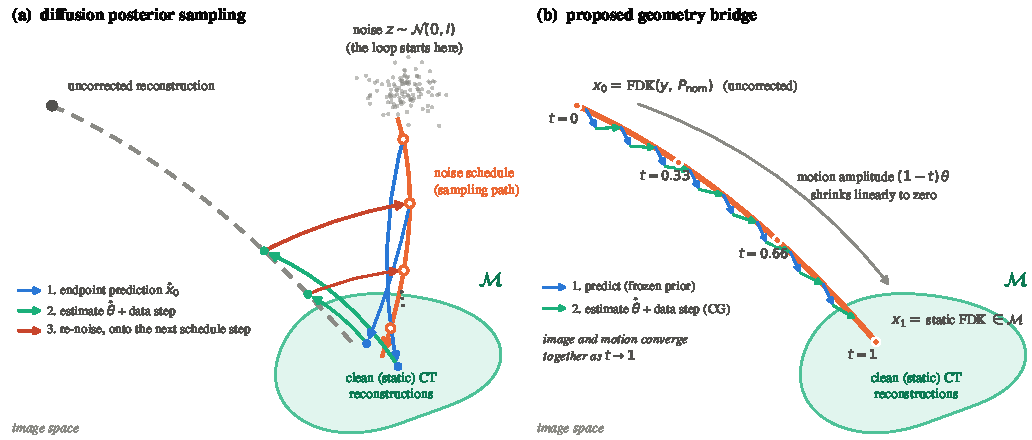
\includegraphics[width=0.95\textwidth]{fig0_manifold.pdf}
\caption{Concept of the proposed method. (a) A conventional generative prior transports
Gaussian noise to the clean-image manifold $\mathcal{M}$ along a fixed noise schedule. In a
DPS-style loop the prior predicts a clean endpoint, the motion and data steps pull the
estimate back toward the partially corrected states, and the result must be re-noised
onto the next schedule step before the prior can act again, so the correction advances
only through repeated departures from $\mathcal{M}$. (b) The geometry bridge makes those
partially corrected states the training path itself: $x_t$ is the FDK reconstruction of
the scan carrying $(1-t)$ of the motion, the path ends on the static FDK, and the
regression target is the analytic tangent $dx_t/dt$. Inference walks the bridge, with the
prior advancing the image, the motion refit on the improved image, and the data step
returning the iterate to the bridge, so that the image and the motion converge together as
$t\to1$.}
\label{fig:manifold}
\end{figure}

The main contributions of this work are as follows. (1) We introduce a 3D flow-matching
prior defined on the geometry bridge and derive its velocity target analytically from the
exact geometry derivative of the forward projector (Sec.~\ref{sec:bridge}). (2) We develop
a plug-and-play predictor-corrector framework that alternates the learned prior, a
hash-encoded motion estimator and a conjugate-gradient data-consistency step, so that the
volume and motion estimates bootstrap one another through progressive joint refinement
(Sec.~\ref{sec:loop}). We evaluate the method on 30 held-out patients under a fully
specified CBCT geometry against representative autofocus and diffusion-based joint
motion-correction approaches (Sec.~\ref{sec:results-cmp}).\footnote{An earlier version of this work, without the
comparative evaluation, was submitted to SPIE Medical Imaging 2027.}

\section{Methods}
\label{sec:method}

\subsection{Problem formulation}
\label{sec:forward}

Let $x$ denote the attenuation volume and $y$ the log-transformed projections acquired over
$V$ views along the nominal circular orbit $\Pnom$. Patient motion displaces view $v$ by a
rigid pose $\theta_v \in \mathbb{R}^6$ (axis-angle rotation and translation), so the true
acquisition geometry is $P(\theta)[v] = \Pnom[v]\,T(\theta_v)$, where $T(\cdot)$ maps a pose
to its rigid transform and $\theta \in \mathbb{R}^{V\times 6}$ collects the per-view poses
into one trajectory. The scan is then $y = A_{P(\theta)}x$, with $A_P$ the cone-beam forward
projector at geometry $P$; we abbreviate $A_{P(\theta)}$ as $A_\theta$ and the FDK
reconstruction at geometry $P(\theta)$ as $\FDK(\theta)$. We seek the volume and the motion
jointly as an approximate solution of
\begin{equation}
\min_{x,\,\theta}\ \tfrac12\,\|A_{P(\theta)}x - y\|_2^2 \;+\; \lambda\,\mathrm{TV}(x)
\;+\; \mathcal{R}(x),
\label{eq:objective}
\end{equation}
where the data term enforces consistency with the measured projections at the current
geometry estimate, the total-variation term suppresses the streaks that survive an imperfect
geometry, and $\mathcal{R}$ is the learned flow-matching prior described next, which enters
the iteration through its velocity field rather than as an explicit penalty. Because of the
SE(3) gauge, any evaluation of a candidate $(x,\theta)$ must first remove the unobservable
global pose; the conventions we use for this are given in Sec.~\ref{sec:protocol}.

\subsection{Flow-matching prior on the geometry bridge}
\label{sec:bridge}

\begin{figure}[H]
\centering
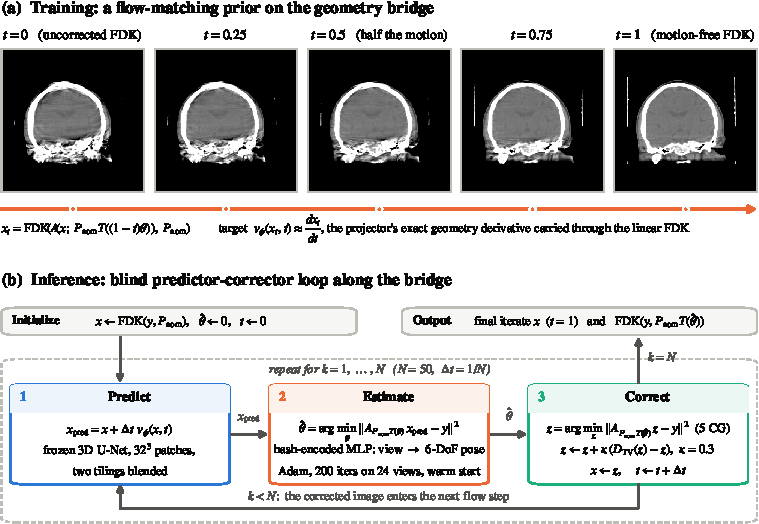
\includegraphics[width=0.80\textwidth]{fig1_method.pdf}
\caption{Overview of the proposed method. (a) The geometry bridge used for training: each
panel is an FDK reconstruction of the same scan re-simulated with $(1-t)$ of the true
motion, and the velocity target $dx_t/dt$ is the projector's exact geometry derivative
carried through the linear FDK. (b) The inference loop of Algorithm~\ref{alg:loop} as a
flowchart: the frozen prior predicts the next image, the motion is re-estimated on that
prediction, and a data-consistency step corrects the image at the new geometry.}
\label{fig:method}
\end{figure}

Flow matching learns a velocity field $v_\phi(x,t)$ that transports one distribution into
another along a prescribed path, by regressing $v_\phi(x_t,t)$ onto the path tangent
$dx_t/dt$. We prescribe the path as the geometry bridge sketched in
Fig.~\ref{fig:manifold}(b) and shown with actual reconstructions in
Fig.~\ref{fig:method}(a): at flow time $t$ the motion is scaled down to $(1-t)\theta$, the
scan is re-simulated at that reduced motion, and the result is reconstructed at the nominal
geometry,
\begin{equation}
y_t = A\!\left(x;\ \Pnom T((1-t)\theta)\right), \qquad
x_t = \FDK(y_t,\ \Pnom).
\label{eq:bridge}
\end{equation}
Since the bridge scales the axis-angle vector, the motion carried by $y_t$ is exactly
$(1-t)\theta$, and the path sweeps the motion amplitude linearly to zero through a sequence
of genuine FDK reconstructions of the same patient scanned with progressively less motion.
Both endpoints follow without any correction term. At $t{=}0$ the re-simulated scan is the
measured one, so $x_0 = \FDK(y,\Pnom)$ is exactly the uncorrected reconstruction from which
inference starts, and at $t{=}1$ the scan is motion-free on the nominal circular,
equiangular orbit, so $x_1$ is exactly the static FDK, the best image this scanner and this
operator can produce of a still patient.

Because FDK is linear in the sinogram and $\Pnom$ does not depend on $t$, the tangent of
this path is available in closed form; the time derivative simply passes through the
reconstruction operator,
\begin{equation}
\frac{dx_t}{dt} = \FDK\!\left(\frac{\partial y_t}{\partial t},\ \Pnom\right),
\qquad
\frac{\partial y_t}{\partial t}
= -\,\frac{\partial A}{\partial P}\Big[x;\ \Pnom T((1-t)\theta)\Big]\cdot \Pnom\,\dot{T}\,\theta,
\label{eq:tangent}
\end{equation}
where $\partial A/\partial P$ is the projector's exact geometry derivative and $\dot T$ the
axis-angle generator. The training loss is the plain regression
$\|v_\phi(x_t,t) - dx_t/dt\|^2$ with $t\sim\mathcal{U}[0,1]$.

This construction is chosen with the inference loop in mind. At every step of the loop the
motion is refit as the trajectory that best explains the projections given the current
image, and the accuracy of that fit is bounded by the quality of the image it is made
against. A prior trained on the bridge moves any partially corrected reconstruction toward
a less corrupted one, which is precisely the improvement the estimator needs, so its
velocity assists motion estimation directly.

The velocity field is a 3D U-Net acting on $32^3$ patches, which keeps memory bounded on a
$256^3$ volume but leaves each patch blind to the rest of the head. Following~\cite{yang25},
every patch therefore receives four conditioning channels besides its own intensities: a
copy of the whole current volume downsampled to the patch size, which conveys the global
anatomy and the overall streak pattern, and three maps holding the absolute $z$, $y$ and
$x$ coordinates of the patch's voxels, which act as a positional encoding. The coordinate
maps let the network relate a patch to its location in the volume and thus to the
downsampled context it is given, so that local texture and global anatomy are combined
consistently across patches.

\subsection{Predictor-corrector inference loop}
\label{sec:loop}

Algorithm~\ref{alg:loop} lists the inference procedure and Fig.~\ref{fig:method}(b)
draws it as a flowchart. The loop starts from
$x = \FDK(y,\Pnom)$ and $\thetahat = 0$ and takes $N{=}50$ Euler steps along the bridge,
each of which is one block-coordinate sweep over Eq.~\eqref{eq:objective}: the prior
moves the image, the motion is re-estimated on the improved image, and the data and TV
terms are enforced at the new geometry.

\begin{algorithm}[H]
\caption{Blind rigid-motion correction along the geometry bridge}
\label{alg:loop}
\begin{algorithmic}[1]
\Require projections $y$, nominal geometry $\Pnom$, frozen prior $v_\phi$, number of steps $N$
\State $x \gets \FDK(y,\Pnom)$,\quad $\thetahat \gets 0$,\quad $t \gets 0$,\quad $\Delta t \gets 1/N$
\For{$k = 1,\dots,N$}
  \State $x_{\mathrm{pred}} \gets x + \Delta t\, v_\phi(x,t)$ \Comment{predict: one Euler step of the prior}
  \State $\thetahat \gets \arg\min_\theta \|A_{\Pnom T(\theta)}\,x_{\mathrm{pred}} - y\|_2^2$ \Comment{estimate: hash-encoded MLP, warm-started Adam}
  \State $z \gets \arg\min_z \|A_{\Pnom T(\thetahat)}\,z - y\|_2^2$ \Comment{correct: five CG iterations}
  \State $z \gets z + \kappa\,(D_{\mathrm{TV}}(z) - z)$ \Comment{relaxed TV update}
  \State $x \gets z$,\quad $t \gets t + \Delta t$
\EndFor
\State \Return final iterate $x$ and $\FDK(y,\Pnom T(\thetahat))$
\end{algorithmic}
\end{algorithm}

\textbf{Predict.} The frozen prior advances the image by one Euler step,
$x_{\mathrm{pred}} = x + \Delta t\,v_\phi(x,t)$, evaluated patch-wise and blended over two
tilings.

\textbf{Estimate.} The motion is then refit by minimizing
$\|A_{\Pnom T(\theta)}\,x_{\mathrm{pred}} - y\|_2^2$ over $\theta$, backpropagating through
the projector's exact geometry gradient. Rather than treating the poses as free per-view
parameters, an MLP reads the normalized view index through a multiresolution hash
encoding~\cite{mueller22} and outputs the 6-DoF pose, so the trajectory is a continuous
function of the view and needs no explicit smoothness penalty. Adam optimizes the encoder
and MLP weights, and its state persists across flow steps so that each refit warm-starts
from the previous one. Fitting against $x_{\mathrm{pred}}$ rather than $x$ matters, because
the accuracy of the fit is bounded by the quality of the image it is made against; as the
prior cleans the iterate, the estimate sharpens, which in turn feeds a cleaner image back to
the prior.

\textbf{Correct.} Finally, a plug-and-play step enforces consistency at $\thetahat$
through five conjugate-gradient (CG) iterations on $\min_z \|A_{\thetahat}z - y\|^2$,
followed by a relaxed total-variation update
$z \leftarrow z + \kappa\,(D_{\mathrm{TV}}(z) - z)$, where $D_{\mathrm{TV}}(z)$ denotes a
TV-denoised copy of $z$. A short CG solve is used rather than a single adjoint step because
the gain from a better $\thetahat$ lies in streaks and edges, which an adjoint step barely
touches. The output becomes the image the prior advances at the next flow time, so the
image and the motion converge together as $t$ runs to 1. The loop returns both the final
iterate $x_t$ and the analytic reconstruction $\FDK(\thetahat)$; the latter contains no
learned component, so it allows the recovered geometry to be verified independently of the
prior.

\subsection{Implementation details}
\label{sec:impl}

The U-Net has base width 32 with channel multipliers $(1,2,4)$, two residual blocks per
level and a time embedding, for 9.9M parameters and five input channels (the patch plus the
four conditioning channels of Sec.~\ref{sec:bridge}). It was trained for 500k iterations
with AdamW, a cosine learning-rate schedule from $10^{-4}$ to $10^{-6}$, EMA 0.999, fp16,
and 64 patches per batch. All projections and backprojections use the differentiable
projector of LEAP~\cite{leap23}; the bridge tangent and the pose gradient are exact
derivatives of that same operator. At inference the estimator runs 200 Adam
iterations per flow step on 24 randomly drawn views, at half volume resolution until
$t=0.5$; the data step uses five CG iterations with the TV relaxation weight
$\kappa = 0.3$ and step size 0.015 over five TV iterations. The source code is available at
\url{https://github.com/dbstjstod1/Flow_matching_motion_3D}.

\section{Experiments}
\label{sec:setup}

\subsection{Data and simulation setup}
\label{sec:data}

We use the CQ500 head CT collection~\cite{cq500}, applying the thin-slice series
selection of~\cite{thies25} (one thin-slice reconstruction per patient, slice-count
outliers removed), which retains 343 patients, of which 150 are used for training, 50 for
validation and 143 for testing, reconstructed at $256^3$ with 1\,mm voxels. Projections are simulated as noiseless line integrals on a finer $612^3$ grid at
0.42\,mm to avoid an inverse crime, through the standard head-CBCT geometry
of~\cite{thies25}: source-isocenter distance 785\,mm,
source-detector distance 1200\,mm, a $700\times500$ detector at 0.64\,mm pixel pitch, and
360 views over a full turn. Photon noise, scatter and beam hardening are not modelled; we
return to this in Sec.~\ref{sec:discussion}. Per-view motion follows the motion model
of~\cite{thies25}: for each DoF, a zero-centred Akima spline~\cite{akima70}, a
piecewise-cubic interpolant that passes through its nodes without the overshoot of a global
spline, is drawn through 10 random nodes; training draws per-DoF amplitudes up to 15\,mm\,/\,20$^\circ$, and evaluation uses one
fixed 10\,mm\,/\,10$^\circ$ pattern per patient.

All amplitudes are peak-to-peak. The evaluation amplitude of 10\,mm\,/\,10$^\circ$
matches that of~\cite{depaepe25}, whose spline control points span $[-5,5]$\,mm and
degrees, and is twice the amplitude at which~\cite{thies25} was evaluated, so all methods
are tested on a deliberately more challenging motion.

\subsection{Evaluation protocol}
\label{sec:protocol}

Following the 30-patient protocol of~\cite{thies25}, we score 30 patients from the held-out
test split, one motion pattern each; every method sees identical (patient, motion draw,
sinogram) triples, so all comparisons are paired. Because of the SE(3) gauge, volumes are
rigidly aligned to the ground truth before PSNR and SSIM are computed, and the scores are
read within the scanner's measured field of view for every method alike; the alignment is
converged and agrees with the gauge fitted directly to $\thetahat$ in the pose domain.

Motion accuracy is measured in two domains. In the projection domain we use the
reprojection error (RPE)~\cite{thies25}, the mean detector displacement induced by the
pose error over a set of points in the head, computed after removing the mean pose offset,
which the SE(3) gauge leaves unobservable and which requires no ground truth to remove. In
the
image domain we compare the reconstruction at the estimated poses against the
ground-truth volume.

We also assess the recovered motion parameters directly. For each of the six degrees of
freedom, the estimated trajectory $\thetahat$ is compared view by view with the true
trajectory $\theta$ after the unobservable global rigid transform has been removed, and
the error is summarized as the mean absolute error per degree of freedom over all views
and patients, separately for the three translations and the three rotations. This
complements the RPE, which folds all six components into a single detector-plane
displacement, by showing whether every component of the motion is recovered.

\subsection{Comparison methods}
\label{sec:baselines}

\paragraph{Learned autofocus~\cite{thies25}.}
The method of Thies et al. casts motion estimation as autofocus with a learned quality
metric as its objective. A quality
network is trained to regress, from the reconstruction of a motion-perturbed scan, a
voxel-wise map of the visual information fidelity (VIF) of that reconstruction relative to
its motion-free counterpart. At test time the network is frozen and serves as the
objective: the spline nodes of the 6-DoF trajectory are optimized by gradient descent to
maximize the predicted quality of the reconstruction, with the gradient flowing through a
differentiable backprojector, and the image returned is the analytic reconstruction at the
estimated poses. No projection-domain data term is involved; the estimate is driven
entirely by the appearance of the reconstruction. We use the authors' publicly released
implementation, with the quality network retrained on our 150 training patients under
their protocol, and the baseline is reconstructed with its own operator throughout.

\paragraph{JRM-ADM~\cite{depaepe25}.}
JRM-ADM, the joint reconstruction and motion estimation adaptive diffusion model of De
Paepe et al., addresses the same coupled problem with a diffusion prior used in the manner of
diffusion posterior sampling. Its prior is a 3D diffusion model of clean head volumes in
the Haar-wavelet domain (W3DM~\cite{wdm24}), and along the sampling trajectory each
clean-volume prediction of the prior is followed by a volume update on a
weighted-least-squares projection residual and a gradient-descent update of the 6-DoF
motion, parameterized by cubic B-spline control points, on the same residual. We run the
authors' publicly released implementation as published, keeping their sampler,
optimizers, motion model and prior unchanged, with the prior retrained on our 150 training
patients under their noise schedule. The method was designed for sparse-view acquisitions;
since full-view data only provide it with more measurements, we apply it to our data
without modification.

\paragraph{Bridge ablation (pixel-linear bridge).}
To isolate what the bridge itself contributes, we trained an identically configured prior,
with the same U-Net, conditioning, $t$-sampling and 500k recipe, on the pixel-linear bridge
$x_t = (1-t)x_0 + t\,x_1$ between the same two endpoints, whose velocity target is the
constant $x_1 - x_0$. Any difference between the two arms is then attributable to the
bridge shape, a curve through actual FDK reconstructions supervised by the exact operator
tangent, rather than to architecture or training.

\section{Results}
\label{sec:results}

\subsection{Performance of the proposed method}
\label{sec:results-main}

\begin{figure}[H]
\centering
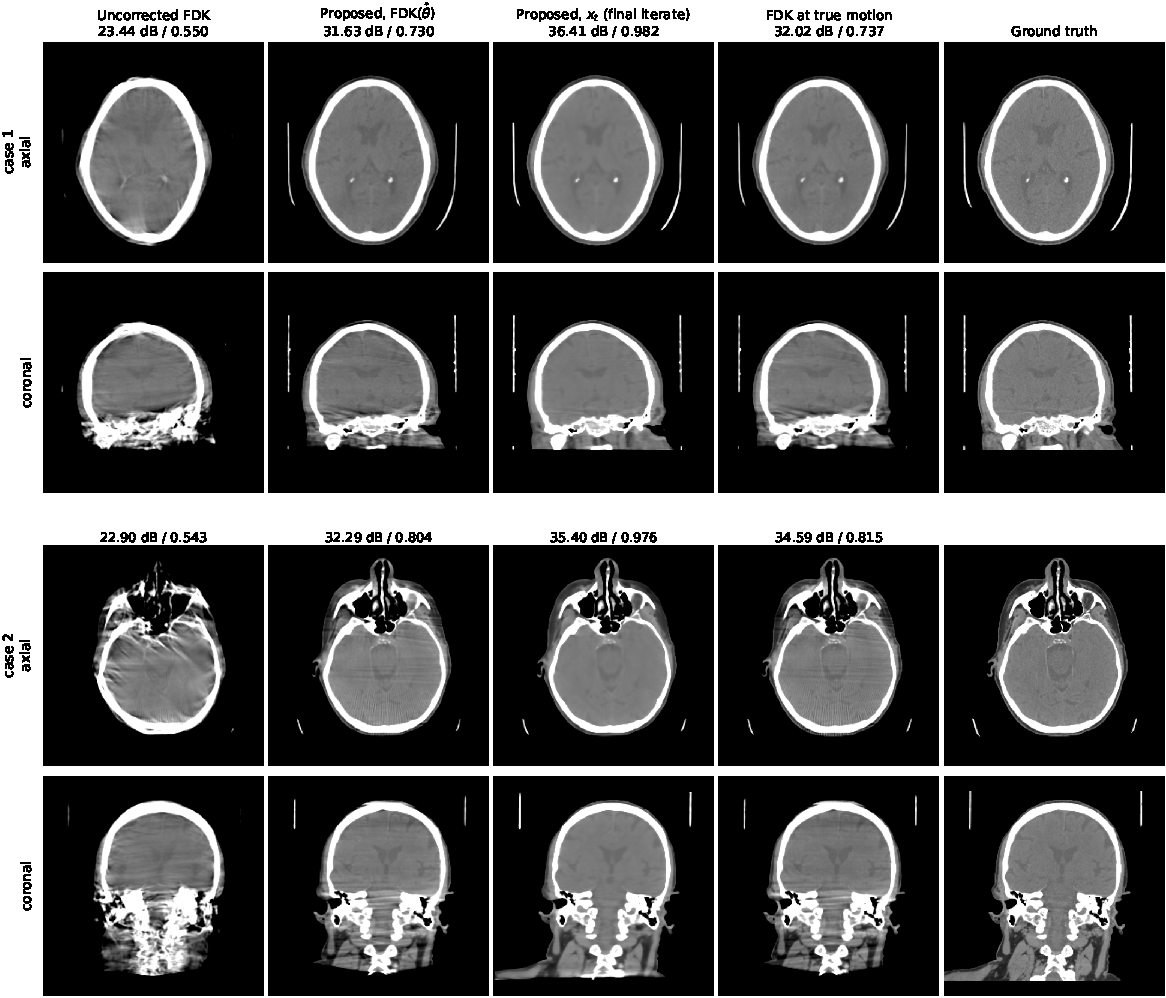
\includegraphics[width=0.92\textwidth]{fig_ours_qual.pdf}
\caption{Two representative test patients at 10\,mm\,/\,10$^\circ$ motion, brain window
(level 40\,/\,width 420\,HU); volumes are rigidly aligned to the ground truth before
display, and labels give PSNR\,/\,SSIM against the ground-truth volume. The fourth column
is the FDK of the same scan at the true motion.}
\label{fig:images}
\end{figure}

\begin{table}[H]
\centering
\caption{Performance of the proposed method on 30 held-out CQ500 patients with Akima
motion at 10\,mm\,/\,10$^\circ$ peak-to-peak. PSNR and SSIM are computed against the
ground-truth volume after rigid alignment, within the measured field of view; RPE is the
reprojection error of~\cite{thies25} with the mean pose offset removed (mean $\pm$
standard deviation).}
\label{tab:main}
\begin{tabular}{lccc}
\toprule
Output & PSNR (dB) & SSIM & RPE (mm) \\
\midrule
Uncorrected FDK & 23.29 $\pm$ 0.93 & 0.546 $\pm$ 0.035 & 6.12 $\pm$ 0.66 \\
FDK($\thetahat$) & 31.80 $\pm$ 0.76 & 0.753 $\pm$ 0.032 & 0.28 $\pm$ 0.09 \\
\textbf{$x_t$ (final iterate)} & \textbf{36.66 $\pm$ 1.58} & \textbf{0.978 $\pm$ 0.008} & \textbf{0.28 $\pm$ 0.09} \\
\bottomrule
\end{tabular}
\end{table}

\begin{figure}[H]
\centering
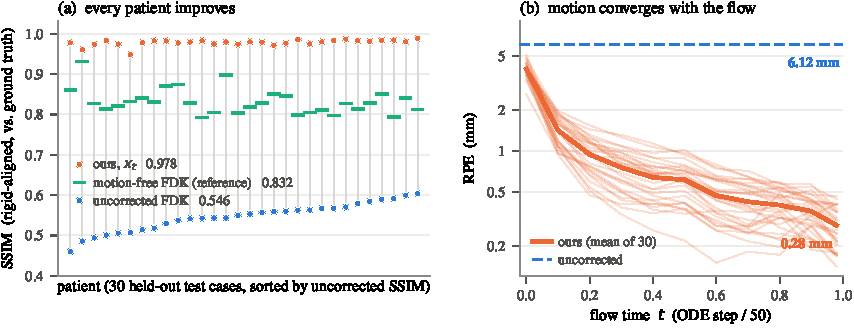
\includegraphics[width=0.78\textwidth]{fig3_quant.pdf}
\caption{Cohort results over 30 held-out patients. (a) Per-patient SSIM; grey stems join
each patient's uncorrected and corrected score. (b) Reprojection error against flow time
(thin: individual patients).}
\label{fig:quant}
\end{figure}

Table~\ref{tab:main} summarizes the proposed method over the cohort, and
Fig.~\ref{fig:quant}(a) shows the per-patient picture. Starting from an uncorrected
reconstruction at 23.29\,dB\,/\,0.546 SSIM, the final iterate reaches
36.66\,dB\,/\,0.978 and improves every one of the 30 patients. As can be seen in
Fig.~\ref{fig:quant}(b), the reprojection error decreases steadily along the flow, from
6.12\,mm to 0.28\,mm at $t{=}1$, so the recovered motion is nearly exact by the end of the
bridge. Inference takes 9.3 minutes per patient on one RTX A6000 GPU
(Sec.~\ref{sec:cost}).

The two outputs of the loop play different roles. FDK($\thetahat$) contains no learned
component, so its quality is evidence about the motion estimate alone, and its remaining
artifacts are those of the analytic operator at the corrected geometry rather than of
residual motion. The final iterate exceeds it by 4.9\,dB and 0.225 SSIM, and it also
exceeds the motion-free FDK of the same scanner (33.11\,dB\,/\,0.832 SSIM on this cohort)
by 3.5\,dB and 0.146 SSIM, because the same loop that corrects the geometry also
regularizes the cone-beam and finite-view artifacts that FDK leaves behind. This is why we
regard the final iterate, rather than an analytic reconstruction, as the primary output,
while FDK($\thetahat$) remains valuable as a learning-free witness of the recovered
geometry. The qualitative results in Fig.~\ref{fig:images} show both roles:
FDK($\thetahat$) is visually indistinguishable from the FDK at the ground-truth motion,
and both retain artifacts that only the final iterate removes.

\FloatBarrier
\subsection{Comparison with other methods}
\label{sec:results-cmp}

\begin{figure}[H]
\centering
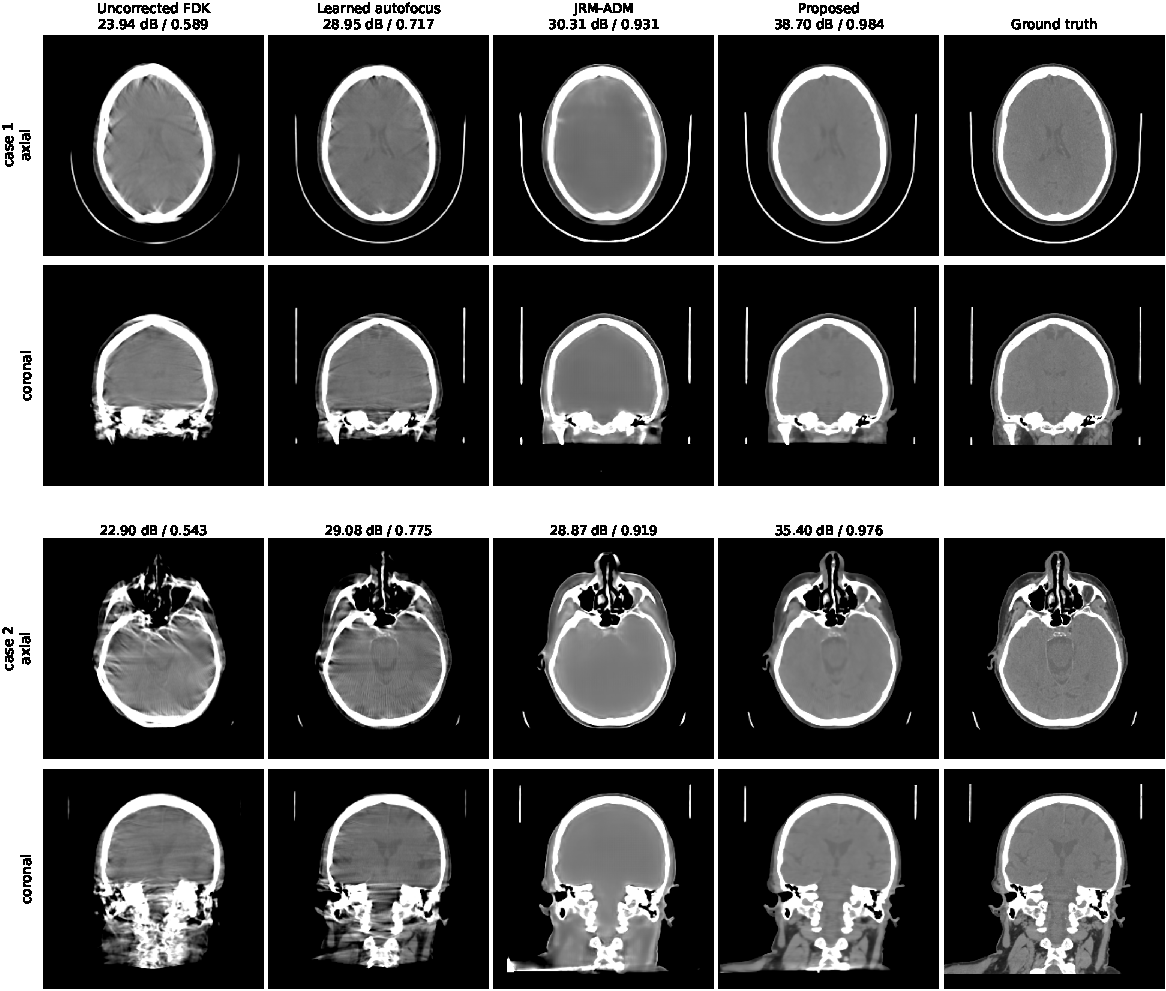
\includegraphics[width=0.80\textwidth]{fig4_bench.pdf}
\caption{Qualitative comparison on two representative test patients, axial and coronal
slices in the brain window; the axial slice of the second case lies at the skull-base level.
All volumes are rigidly aligned to the ground truth before slicing, and labels give
PSNR\,/\,SSIM against the ground truth.}
\label{fig:bench}
\end{figure}

\begin{table}[H]
\centering
\caption{Comparison with other methods on the same 30 patients, under the conventions
of Table~\ref{tab:main}. All learned components were retrained on the same 150 training
patients and evaluated on identical (patient, motion, sinogram) triples. The pixel-linear row is the bridge
ablation discussed at the end of this section.}
\label{tab:cmp}
\begin{tabular}{lccc}
\toprule
Method & PSNR (dB) & SSIM & RPE (mm) \\
\midrule
Learned autofocus~\cite{thies25} & 29.22 $\pm$ 1.11 & 0.727 $\pm$ 0.032 & 2.26 $\pm$ 0.52 \\
JRM-ADM~\cite{depaepe25} & 29.64 $\pm$ 2.64 & 0.912 $\pm$ 0.038 & 0.84 $\pm$ 0.55 \\
Proposed, FDK($\thetahat$) & 31.80 $\pm$ 0.76 & 0.753 $\pm$ 0.032 & 0.28 $\pm$ 0.09 \\
Proposed, pixel-linear bridge (ablation) & 35.29 $\pm$ 2.28 & 0.966 $\pm$ 0.015 & 0.42 $\pm$ 0.17 \\
\textbf{Proposed, $x_t$ (final iterate)} & \textbf{36.66 $\pm$ 1.58} & \textbf{0.978 $\pm$ 0.008} & \textbf{0.28 $\pm$ 0.09} \\
\bottomrule
\end{tabular}
\end{table}

Table~\ref{tab:cmp} compares the proposed method with the two comparison methods, and
Fig.~\ref{fig:bench} shows two patients. Against the learned autofocus of Thies et al.~\cite{thies25}, the proposed
loop recovers the motion more accurately, with an RPE of 0.28\,mm
against 2.26\,mm, lower on every one of the 30 patients ($p=1.7\times10^{-6}$). The
difference carries through the analytic reconstruction: FDK($\thetahat$), which shares the
baseline's output type and contains no learned component, exceeds the autofocus output by
2.6\,dB (30/30) and 0.026 SSIM (23/30, $p=1.5\times10^{-4}$), so the advantage in motion
accuracy is visible even before the prior contributes to the image. The final iterate then
adds 4.9\,dB and 0.225 SSIM on top of that, surpassing the autofocus output on all 30
patients in both metrics. As can be seen in Fig.~\ref{fig:bench}, the autofocus baseline
removes much of the motion but keeps residual streaks, whereas the final iterate recovers
both geometry and texture. Re-scoring all outputs inside a body region of interest that
excludes the air background and the patient table preserves every ordering and
significance in Table~\ref{tab:cmp}.

\begin{figure}[H]
\centering
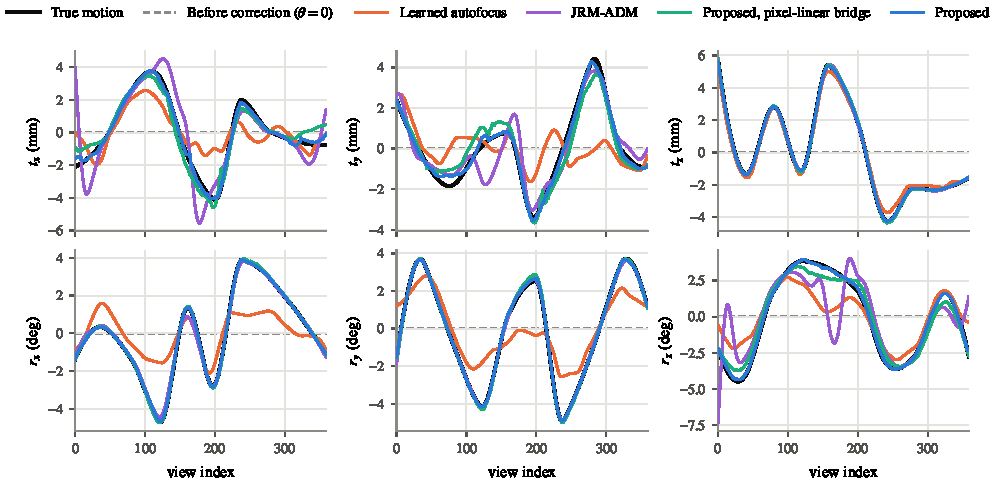
\includegraphics[width=\textwidth]{fig_motion.pdf}
\caption{Recovered motion of one test patient (the first case of Fig.~\ref{fig:bench}).
Each panel shows one degree of freedom against the view index: the true trajectory, the
state before correction ($\theta=0$), and the trajectory recovered by each method, all on
the zero-mean gauge. Translations in mm, rotations in degrees.}
\label{fig:motion}
\end{figure}

\begin{table}[H]
\centering
\caption{Per-DoF mean absolute error of the recovered motion over the 30 patients, on the
zero-mean gauge. Translations in mm, rotations in degrees.}
\label{tab:dof}
\small
\begin{tabular}{lcccccc}
\toprule
Method & $t_x$ & $t_y$ & $t_z$ & $r_x$ & $r_y$ & $r_z$ \\
\midrule
Uncorrected & 1.93 & 2.08 & 1.95 & 2.01 & 1.90 & 2.17 \\
Learned autofocus~\cite{thies25} & 1.30 & 1.33 & 0.36 & 0.95 & 0.98 & 1.09 \\
JRM-ADM~\cite{depaepe25} & 2.17 & 1.97 & 0.06 & 0.09 & 0.07 & 0.68 \\
Proposed, pixel-linear bridge (ablation) & 0.71 & 0.69 & 0.04 & 0.04 & 0.05 & 0.40 \\
\textbf{Proposed} & \textbf{0.79} & \textbf{0.78} & \textbf{0.03} & \textbf{0.04} & \textbf{0.04} & \textbf{0.23} \\
\bottomrule
\end{tabular}
\end{table}

Fig.~\ref{fig:motion} traces the six motion parameters of one patient through the scan,
before correction and as recovered by each method, and Table~\ref{tab:dof} gives the
corresponding per-DoF errors over the cohort. The proposed loop follows the true
trajectory closely in every component, including the two that cone-beam geometry
constrains least: the in-plane translations, one component of which lies along the beam
in every view, and the rotation about the gantry axis, which is nearly equivalent to a
shift of the view angle. The autofocus baseline recovers the general shape of the
trajectory but underestimates its amplitude, and its residual concentrates in exactly
those components. Over the cohort, the proposed method brings the per-component error
from about 2\,mm and 2$^\circ$ before correction down to at most 0.79\,mm and
0.23$^\circ$, whereas the autofocus baseline remains near 1.3\,mm and 1$^\circ$ in the
weakly constrained components. The pixel-linear arm is comparable to the proposed prior on the
translations and less accurate on the gantry-axis rotation, consistent with its RPE.
JRM-ADM recovers the axial translation and the two out-of-plane rotations about as well
as the proposed method and is less accurate on the gantry-axis rotation, yet its in-plane
translation error of about 2.1\,mm exceeds the uncorrected value despite an RPE of
0.84\,mm. Its per-view translation drifts
along the beam direction, which the projections do not constrain; a fixed-axis error sees
that drift, whereas the detector-plane RPE does not.

JRM-ADM, run as published on our data (Sec.~\ref{sec:baselines}), recovers the motion
accurately, with an RPE of 0.84\,mm against 2.26\,mm for the autofocus baseline, and the
analytic
reconstruction at its poses reaches 29.45\,dB\,/\,0.715, behind our
FDK($\thetahat$) by 2.3\,dB (28/30, $p=1.6\times10^{-7}$). Its final output,
however, reaches only 29.64\,dB\,/\,0.912, which is 7.0\,dB
and 0.066 SSIM behind our final iterate (30/30, $p=1.9\times10^{-9}$); as can be seen
in Fig.~\ref{fig:bench}, it removes the motion but returns an over-smoothed volume in
which fine texture is lost. The loss is most visible in soft tissue: the grey-white matter
differentiation and the low-contrast structures that our final iterate restores are
flattened into a nearly uniform parenchyma, so its soft-tissue restoration is markedly
weaker despite the accurate motion estimate. The difference between the two methods
therefore lies mainly in the prior and in how the loop applies it, rather than in the
motion estimate.

The pixel-linear row of Table~\ref{tab:cmp} isolates what the bridge itself contributes. The
pixel-linear arm, trained with an identical recipe between identical endpoints, lands
1.38\,dB and 0.012 SSIM behind the geometry bridge (27/30 patients,
$p=1.6\times10^{-7}$) and recovers the motion less accurately (0.42 against 0.28\,mm),
even though the estimator, the data step and the schedule are identical in the two arms.
The margin is larger than the two priors show in isolation, since a slightly better
intermediate image buys a better motion fit, which buys a cleaner data step, compounding
over the 50 sweeps. In Fig.~\ref{fig:motion} the two bridge-trained arms track the
trajectory similarly, the geometry bridge more closely on the gantry-axis rotation.

\FloatBarrier
\subsection{Computational cost}
\label{sec:cost}

\begin{table}[H]
\centering
\caption{Computational cost per patient on one NVIDIA RTX A6000 GPU, for the
configurations used in the comparison (360 views, $256^3$ volume). The third column counts
projector-gradient evaluations in full-view equivalents, one unit being one pass over all
360 views (an evaluation on 24 views counts 24/360); counts are approximate. The runtime of
the learned autofocus is the value stated by its authors.}
\label{tab:cost}
\small
\begin{tabular}{lccc}
\toprule
Method & Network calls & Full-view projector-gradient evaluations & Time \\
\midrule
Learned autofocus~\cite{thies25} & 100 & $\sim$100 & $<2$\,min \\
JRM-ADM~\cite{depaepe25} & 100 & $\sim$1{,}600 & 4.6\,h \\
Proposed & 50 & $\sim$900 & 9.3\,min \\
\bottomrule
\end{tabular}
\end{table}

Table~\ref{tab:cost} summarizes the cost of the three methods. In every case the
projector, not the network, dominates: each method spends most of its time in
projection and backprojection operations, either to fit the motion or to enforce data
consistency. The learned autofocus is the fastest because it performs a single descent of
100 iterations, each of which reconstructs the volume from all views and backpropagates
the quality metric through that reconstruction, one full-view evaluation per iteration,
and returns an analytic image. Our loop takes 9.3 minutes, of which roughly
80\% is spent in the motion estimator; the estimator refits the trajectory at every one
of the 50 flow steps, but on 24 randomly drawn views per iteration and at half resolution
for the first half of the bridge, so its 10{,}000 Adam iterations amount to about 670
full-view equivalents, to which the 250 CG iterations of the data step add 250. JRM-ADM
performs about 1{,}600 such evaluations, since each of its 100 diffusion steps runs 10 to
15 RMSprop iterations on the volume and 5 to 10 on the motion, every one over all 360
views. The evaluation count is thus less than twice ours, and the remaining factor in its
30-fold longer runtime is the cost per evaluation of its projector implementation, which
processes the views in chunks and passes a $224^3$ volume and its wavelet prior through
every step. The count itself reflects its design target: at the 20 to 60 views of the
sparse-view protocol it was developed for, the same iteration counts are six to eighteen
times cheaper, so the runtime comparison is specific to the full-view protocol used here.

\FloatBarrier
\section{Discussion}
\label{sec:discussion}

What flow matching contributes to this problem is the freedom to choose the transport
path. Trained along the geometry bridge, the prior is defined exactly on the states a
blind correction loop traverses, and the bridge ablation makes the value of that choice
concrete. The comparison with the autofocus baseline draws a complementary lesson. At this
motion amplitude, both its estimator and ours recover the geometry well enough that their
analytic reconstructions differ by far less than either differs from the final iterate,
so the practically relevant distinction between methods has shifted from how well the
motion is estimated to what kind of image is returned. The comparison with JRM-ADM points
the same way: its motion estimate is competitive, but its output loses the texture that
the bridge-trained prior preserves. An analytic reconstruction
inherits the ceiling of its operator; the loop's own iterate does not, and ours ends above
the motion-free analytic reference. Returning both outputs keeps the method auditable, since
the analytic one certifies the geometry that the learned one builds on.

Several limitations bound these claims. The projections are simulated noiseless line
integrals, so photon statistics, scatter and beam hardening, all present in real
acquisitions, are outside the present evidence, and no public head-CBCT projection data
with genuine patient motion exists to our knowledge; clinical validation is the essential
next step. The motion model is rigid, which suits the skull but not the mandible or the
neck. The autofocus baseline runs the authors' code with a quality network retrained on our
data at twice the motion amplitude of its published evaluation, and its residual RPE in our
setting is above the published value, so its motion accuracy should be read as
conservative. Finally, at 9.3 minutes per patient the
method is slower than the autofocus baseline (Sec.~\ref{sec:cost}), and the estimator, which dominates our budget, is
the natural target for acceleration before interventional use can be considered.

\section{Conclusion}
\label{sec:conclusion}

We presented a blind rigid-motion correction method for head CBCT whose prior is trained
along the very path a correction loop traverses, with a closed-form velocity target
derived from the projector's exact geometry derivative. On 30 held-out patients the loop
recovered the motion to 0.28\,mm reprojection error and improved every case, and paired
comparisons against a learned autofocus method and a diffusion-based joint method showed
consistent gains in both motion accuracy and image quality, with a bridge ablation
attributing part of the margin to the bridge itself.
Since the final iterate exceeds even the motion-free analytic reference, further progress
at this amplitude lies with the reconstruction rather than with the motion estimate.

\begin{thebibliography}{17}\small

\bibitem{sisniega17} A.~Sisniega, J.~W. Stayman, J.~Yorkston, J.~H. Siewerdsen, and
W.~Zbijewski, ``Motion compensation in extremity cone-beam CT using a penalized image
sharpness criterion,'' \emph{Phys. Med. Biol.} \textbf{62}(9), 3712--3734 (2017).

\bibitem{thies25} M.~Thies et al., ``A gradient-based approach to fast and accurate head
motion compensation in cone-beam CT,'' \emph{IEEE Trans. Med. Imaging} \textbf{44}(2),
1098--1109 (2025).

\bibitem{huang22} H.~Huang, J.~H. Siewerdsen, W.~Zbijewski, C.~R. Weiss, T.~Ehtiati, and
A.~Sisniega, ``Reference-free learning-based similarity metric for motion compensation in
cone-beam CT,'' \emph{Phys. Med. Biol.} \textbf{67}(12), 125020 (2022).

\bibitem{ko21} Y.~Ko, S.~Moon, J.~Baek, and H.~Shim, ``Rigid and non-rigid motion artifact
reduction in X-ray CT using attention module,'' \emph{Med. Image Anal.} \textbf{67}, 101883
(2021).

\bibitem{pnp13} S.~V. Venkatakrishnan, C.~A. Bouman, and B.~Wohlberg, ``Plug-and-play priors
for model based reconstruction,'' in \emph{IEEE GlobalSIP}, 945--948 (2013).

\bibitem{dds24} H.~Chung, S.~Lee, and J.~C. Ye, ``Decomposed diffusion sampler for
accelerating large-scale inverse problems,'' in \emph{ICLR} (2024).

\bibitem{depaepe25} A.~De Paepe, A.~Bousse, C.~Phung-Ngoc, Y.~Mellak, and D.~Visvikis,
``Adaptive diffusion models for sparse-view motion-corrected head cone-beam CT,''
\emph{IEEE Trans. Radiat. Plasma Med. Sci.} (2025); arXiv:2504.14033.

\bibitem{lipman23} Y.~Lipman, R.~T.~Q. Chen, H.~Ben-Hamu, M.~Nickel, and M.~Le, ``Flow
matching for generative modeling,'' in \emph{ICLR} (2023).

\bibitem{indi23} M.~Delbracio and P.~Milanfar, ``Inversion by direct iteration: an
alternative to denoising diffusion for image restoration,'' \emph{Trans. Mach. Learn. Res.}
(2023).

\bibitem{albergo23} M.~S. Albergo, M.~Goldstein, N.~M. Boffi, R.~Ranganath, and
E.~Vanden-Eijnden, ``Stochastic interpolants with data-dependent couplings,'' arXiv:2310.03725
(2023).

\bibitem{i2sb23} G.-H. Liu, A.~Vahdat, D.-A. Huang, E.~A. Theodorou, W.~Nie, and
A.~Anandkumar, ``I$^2$SB: image-to-image Schr\"odinger bridge,'' in \emph{ICML} (2023).

\bibitem{yang25} T.~Yang, J.~Hu, J.~A. Fessler, and L.~Shen, ``Local patches meet global
context: scalable 3D diffusion priors for computed tomography reconstruction,''
arXiv:2512.18161 (2025).

\bibitem{mueller22} T.~M\"uller, A.~Evans, C.~Schied, and A.~Keller, ``Instant neural
graphics primitives with a multiresolution hash encoding,'' \emph{ACM Trans. Graph.}
\textbf{41}(4), 102 (2022).

\bibitem{leap23} H.~Kim and K.~Champley, ``Differentiable forward projector for X-ray
computed tomography,'' arXiv:2307.05801 (2023); LEAP,
\url{https://github.com/LLNL/LEAP}.

\bibitem{cq500} S.~Chilamkurthy et al., ``Deep learning algorithms for detection of critical
findings in head CT scans: a retrospective study,'' \emph{The Lancet} \textbf{392}(10162),
2388--2396 (2018).

\bibitem{akima70} H.~Akima, ``A new method of interpolation and smooth curve fitting based on
local procedures,'' \emph{J. ACM} \textbf{17}(4), 589--602 (1970).

\bibitem{wdm24} P.~Friedrich, J.~Wolleb, F.~Bieder, A.~Durrer, and P.~C. Cattin, ``WDM: 3D
wavelet diffusion models for high-resolution medical image synthesis,'' in \emph{MICCAI
Workshop on Deep Generative Models}, 11--21 (2024).

\end{thebibliography}

\end{document}
